\section{Spin Glass}

\subsection{Order parameters}
Last class we introduced the Edwards-Anderson order parameter:
\begin{equation}
    Q_{EA} = \frac{1}{N}\sum_{i=1}^N\avg{\sigma_i}^2
\end{equation}
we then had the order parameter quantifying overlap:
\begin{equation}
    q_{\sigma\tau} = \frac{1}{N}\sum_{i=1}^N \sigma_i\tau_i
\end{equation}
and the average:
\begin{equation}
    Q_{\alpha\beta} = \frac{1}{N}\sum_{i=1}^N \avg{\sigma_i}_\alpha \avg{\sigma_i}_\beta
\end{equation}
where the $\avg{\cdot}_\alpha$ denotes an average over a pure state $\alpha$. 

In a glass, there is no spatial order. But, if we think about something that is frozen, if I look at a single spin and watch it for a very long time, it doesn't flip. So, order in a glass is really a statement about temporal order. The way to measure this would be to take the thermal average of a single spin $i$. If at this point I average over spins, I get zero (as there is no spatial order). But if I square it and then average, I get a finite value.

Generalizing $Q_{EA}$, we consider that our system may break ergodicity. It doesn't explore all of phase space; it gets stuck. There can be multiple states that survive for long times and are different. That said, they could potentially overlap. Thus there is an overlap matrix $Q_{\alpha\beta}$. If we take the configuration and break it up, there may be multiple pure states $\alpha, \beta$ and then there is some overlap between these states. We do the thermal average over a single site for two pure states, multiply and then take the sum.

To be more precise, when we take this thermal average, we consider:
\begin{equation}
    Q_{\alpha\beta} = \frac{1}{N}\sum_i \frac{1}{Z_\alpha}\int_{\sigma \in \alpha}\mathcal{D}\sigma \sigma_i e^{-H(\sigma)}\frac{1}{Z_\beta}\int_{\tau \in \beta} \mathcal{D}\tau \tau_i e^{-H(\tau)} = \frac{1}{Z_\alpha Z_\beta}\int_\alpha \mathcal{D}\sigma\int_{\beta}\mathcal{D}\tau q_{\sigma\tau}e^{-H(\sigma)}e^{-H(\tau)}
\end{equation}
For a paramagnet we get $Q_{\alpha\alpha} = 0$, and for a frozen state we get $Q_{\alpha\alpha}=1$. We now consider the overlap distribution:
\begin{equation}
    P(q) = \frac{1}{Z^2}\int \mathcal{D}\sigma\mathcal{D}\tau e^{-H(\sigma)-H(\tau)}\delta(q - q_{\alpha\tau})
\end{equation}
For a ferromagnet, we have two equal delta peaks when $q = \pm m^2$. 

\begin{center}
    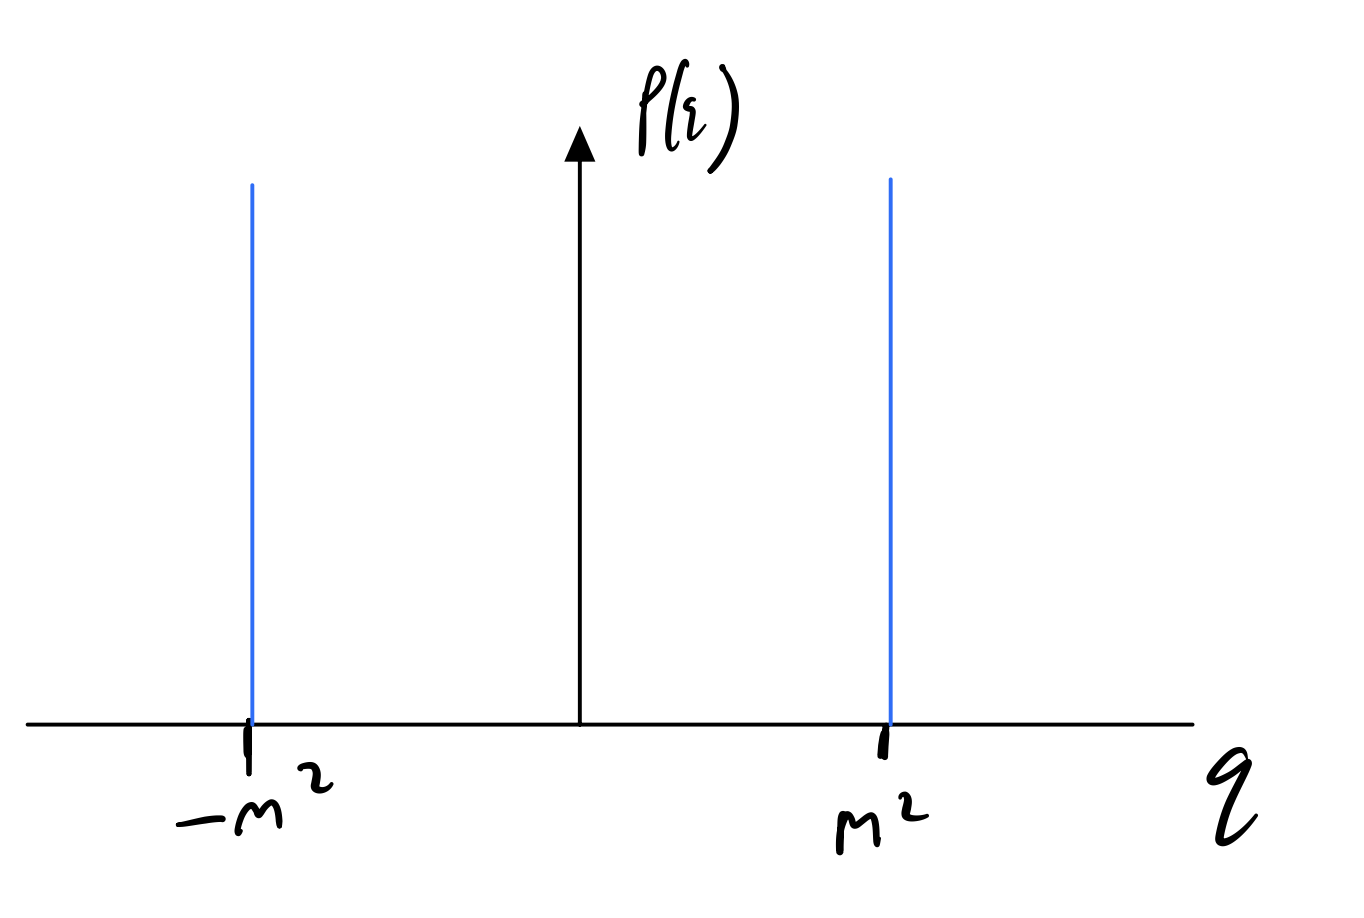
\includegraphics[scale=0.3]{Lectures/Figures/lec14-fmdist.png}
\end{center}

But note that there is generically no reason that this distribution would just be delta functions. Generically, we have delta functions + continuum part. When we find this, we have replica symmetry breaking. The two ferromagnet states have a replica symmetry, but with a continuum no such symmetry is present.

\subsection{Sherrington-Kirepatrick model}
We consider the Hamiltonian:
\begin{equation}
    H = \sum_{i,j=1}^N J_{ij}\sigma_i\sigma_j
\end{equation}
where the $J_{ij}$ are independent random variables:
\begin{equation}
    J_{ij} = \pm \frac{J}{\sqrt{N}}.
\end{equation}
This is a mostly solvable model, coming from the infinite range coupling. Note that even in a model as simple as this one, we have hidden broken symmetries and interesting phenomenology. While we are on the topic of Nobel prizes, this model was also used by Hopfield. He thought about the fact that we could use this model as a memory; if we chose $J_{ij} = \xi_i\xi_j$ with $\xi$ a vector. Then, notice that our Hamiltonian would be minimized with this choice when $\sigma = \xi$ (just a ferromagnet that's been rotated).

\subsection{$p$-spin spherical model}
The model we will actually discuss looks more complicated, but is actually easier:
\begin{equation}
    H = -\sum_{1 \leq i_2 < i_2 < \ldots < i_p \leq N} J_{i_1, \ldots, i_p}\sigma_{i_1}\sigma_{i_2}, \ldots \sigma_{i_p}
\end{equation}
where we consider $p \geq 3$. This is a $p$-spin spherical model (think about the entire set of spins as a vector), with $\frac{1}{N}\sum_{i}\sigma_i^2 = 1$. Each site $i$ has a real-valued spin. The $J$s are drawn from the Gaussian probability distribution:
\begin{equation}
    P(J) = \exp(-\frac{1}{2}J^2\frac{2N^{p-1}}{p!})
\end{equation}
where we note that $\sqrt{\bar{J}^2} \sim \frac{1}{N^{\frac{p-1}{2}}}$. Looking at the averaged $Z$ (for $p=3$):
\begin{equation}
    \overline{Z} = \int \mathcal{D}\sigma\int \prod_{i < j < k} dJ_{ijk}\exp(-\left(J_{ijk}^2\frac{N^{p-1}}{p!} + \beta J_{ijk}\sigma_i\sigma_j\sigma_k\right)) = \int \mathcal{D}\sigma\exp(\frac{\beta^2}{4N^{p-1}}p!\sum_i \sigma_i^2 \sum_j \sigma_j^2 \sum_k \sigma_k^2)
\end{equation}
Each of these sums now just gives $1$, so with the identity $p!\sum_{i>j>k} = \sum_{ijk}$, we just get the surface area of the surface:
\begin{equation}
    \overline{Z} = \exp(\frac{N\beta^2}{4})\Omega
\end{equation}
where $\Omega$ is the solid angle. Now consider $n$ replica version:
\begin{equation}
    \overline{Z^n} = \int \mathcal{D}\sigma_i^\alpha \prod_{ijk}\int dJ_{ijk}\exp(-\frac{J^2N^{p-1}}{p!} + J_{ijk}\beta\sum_{\alpha}^n \sigma_i^\alpha \sigma_j^\alpha \sigma_k^\alpha) = \int \mathcal{D}\sigma \exp(\frac{\beta^2}{4N^{p-1}}\sum_{\alpha,\beta=1}^n \left(\sum_i \sigma_i^\alpha \sigma_i^\beta\right)^p )
\end{equation}
Now we have an overlap matrix! Let us call it:
\begin{equation}
    Q_{\alpha\beta} = \frac{1}{N}\sum_i \sigma^\alpha_i \sigma^\beta_i
\end{equation}
with $Q_{\alpha\alpha} = 1$. How do we deal with this integral? We've seen this a few things, and now what we will do is to introduce an auxilary field. We introduce the trivial statement:
\begin{equation}
    1 = \int dQ_{\alpha\beta}\delta(NQ_{\alpha\beta} - \sum_i \sigma_i^\alpha \sigma_i^\beta) = \int \mathcal{D}\lambda_{ab}e^{-\lambda(NQ_{\alpha\beta} - \sigma_i^\alpha\sigma_j^\beta)}
\end{equation}
But now doing the trick:
\begin{equation}
    \delta(x) = \int dk e^{ikx}
\end{equation}
So by exponentiating the $1$, we can introduce the auxilary field $Q$:
\begin{equation}
    \overline{Z^n} = \int \mathcal{D}Q_{\alpha\beta}\mathcal{D}\lambda_{\alpha\beta}\mathcal{D}\sigma \exp(\frac{\beta^2 N}{4}\sum_{\alpha\beta}Q^p_{\alpha\beta} + N\sum_{\alpha\beta}\lambda_{\alpha\beta}Q_{\alpha\beta} - \sum_i \sum_{\alpha\beta}\sigma_i^\alpha \lambda_{\alpha\beta}\sigma_i^\beta)
\end{equation}
So then:
\begin{equation}
    \overline{Z^n} = \int \mathcal{D}Q_{\alpha\beta}\mathcal{D}\lambda_{\alpha\beta}\exp(-NS(Q, \lambda))
\end{equation}
where:
\begin{equation}
    S(Q, \lambda) = - \frac{\beta}{4}\sum_{\alpha\beta}Q_{\alpha\beta}^p - \sum_{\alpha\beta}\lambda_{\alpha\beta}Q_{\alpha\beta} - \frac{1}{2}\log\det(2\lambda_{\alpha\beta})
\end{equation}
there are no longer fluctuations of spins, but now have two fields. We have an important factor of $N$; this tells us the solution of this problem should be the saddle point of $S$, for everything away from the saddle point becomes exponentially suppressed. We need to consider the limits $n \to 0$ (we are interested in this because $F = \log Z = \lim_{n \to 0}\frac{Z^n - 1}{n}$), $N \to \infty$ (we want a large number of spins/system size, and want $N \to \infty$ so the saddle point is the solution). Then:
\begin{equation}
    -\beta F = \lim_{N \to \infty}\lim_{n \to 0}\frac{1}{nN}\int \mathcal{D}Q\mathcal{D}\lambda e^{-NS}
\end{equation}
The number of independent elements in $Q_{\alpha\beta}$ are $\frac{n(n-1)}{2}$, which as $n \to 0$ becomes negative. This is strange, but we press on - we will do this by interchanging the order of limits. We consider (to obtain the saddle point):
\begin{equation}
    \dpd{}{\lambda_{\alpha\beta}}\left[-\lambda_{\alpha\beta}Q_{\alpha\beta} + \frac{1}{2}\log \det(2\lambda)\right] = 0 \implies -Q_{\alpha\beta} + \frac{1}{2}(\lambda^{-1})_{\alpha\beta} = 0 \implies Q^{-1} = 2\lambda
\end{equation}
Thus replacing the $N \to \infty$ limit integral with the saddle point value:
\begin{equation}
    F = \lim_{n \to \infty} -\frac{1}{2\beta n}\left[\frac{\beta^2}{2}\sum_{\alpha\beta}Q^p_{\alpha\beta} + \log \det Q\right]
\end{equation}
If we now minimize w.r.t $Q$:
\begin{equation}
    0 = \dpd{F}{Q} = \frac{\beta^2 p}{2}Q_{\alpha\beta}^{p-1} + Q^{-1}_{\alpha\beta}
\end{equation}
What do we know? We know $Q_{\alpha\alpha} = 1$. Since there is nothing to distinguish the replicas (i.e. if the model is replica-symmetric) then we would say that all the off-diagonal entries of $Q$ are the same, and equal to some value $q_0$. Then, writing:
\begin{equation}
    Q_{ab} = q_0 + (1 - q_0)\delta_{ab}
\end{equation}
it is clear that:
\begin{equation}
    Q_{ab}^{-1} = \frac{1}{1-q_0}\delta_{ab} - \frac{q_0}{(1-q_0)[1 + (n-1)q_0]}
\end{equation}
here, it's a bit interesting that the $n$ shows up, and I can begin to compute this in the $n \to 0$ limit:
\begin{equation}
    \lim_{n \to 0} \dpd{F}{Q} = \frac{\beta^2 p}{2}q_0^{p-1} - \frac{q_0}{(1-q_0)^2} = 0
\end{equation}
This has two solutions. $q_0 = 0$, which is the paramagnetic, and the pair of solutions:
\begin{equation}
    q_0^{p-2}(1-q_0)^2 = \frac{2}{p\beta^2}
\end{equation}
This is a replica-symmetric solution. It has the unfortunate problem of not being stable. While it is a solution, it we look perturbatively about this solution, e.g. break the system into many pieces, we see that the energy is decreased. Another way to see the instability; it has to not just be a saddle point/extremum, but also a minimum. This requires the eigenvalues to be positive definite.

What does this mean? We still know that everything is dominated by a saddle pont, and just need to find what it is. Let's think about the average/first moment:
\begin{equation}
    q^{(1)} = \bar{Q_{\alpha\beta}}= \lim_{n\to 0} \int \mathcal{D}Q_{\alpha\beta}Q_{\alpha\beta}e^{-NS(Q_{\alpha\beta})}
\end{equation}
what happens when we average over saddle points? When we look at the $\alpha, \beta$s, we have to think about which ones we take. Eventually, this turns into:
\begin{equation}
    \bar{Q_{\alpha\beta}}= \lim_{n \to 0}\frac{2}{n(n-1)}\sum_{\alpha>\beta}Q_{\alpha\beta}
\end{equation}
This average is the first moment, and of course we can generate the $k$th moment, which gives:
\begin{equation}
    q^{(k)} = \lim_{n \to 0}\frac{2}{n(n-1)}\sum_{\alpha\beta}\overline{Q_{\alpha\beta}^k}
\end{equation}
the higher moments are more and more sensitive to the broken symmetry. We then get the distribution:
\begin{equation}
    \bar{P}(q) = \lim_{n \to 0}\frac{2}{n(n-1)}\sum_{a > b}\delta(q - Q_{ab})
\end{equation}
The distribution is governed by the fact that the likely overlap is is given by a value of $q$. Working with this probability distribution, we cab rewrite it as:
\begin{equation}
    P(q) = (1-m)\delta(q - q_1) - m\delta(q - q_0)
\end{equation}
with $0 < m < 1$. We then have the distribution:

\begin{center}
    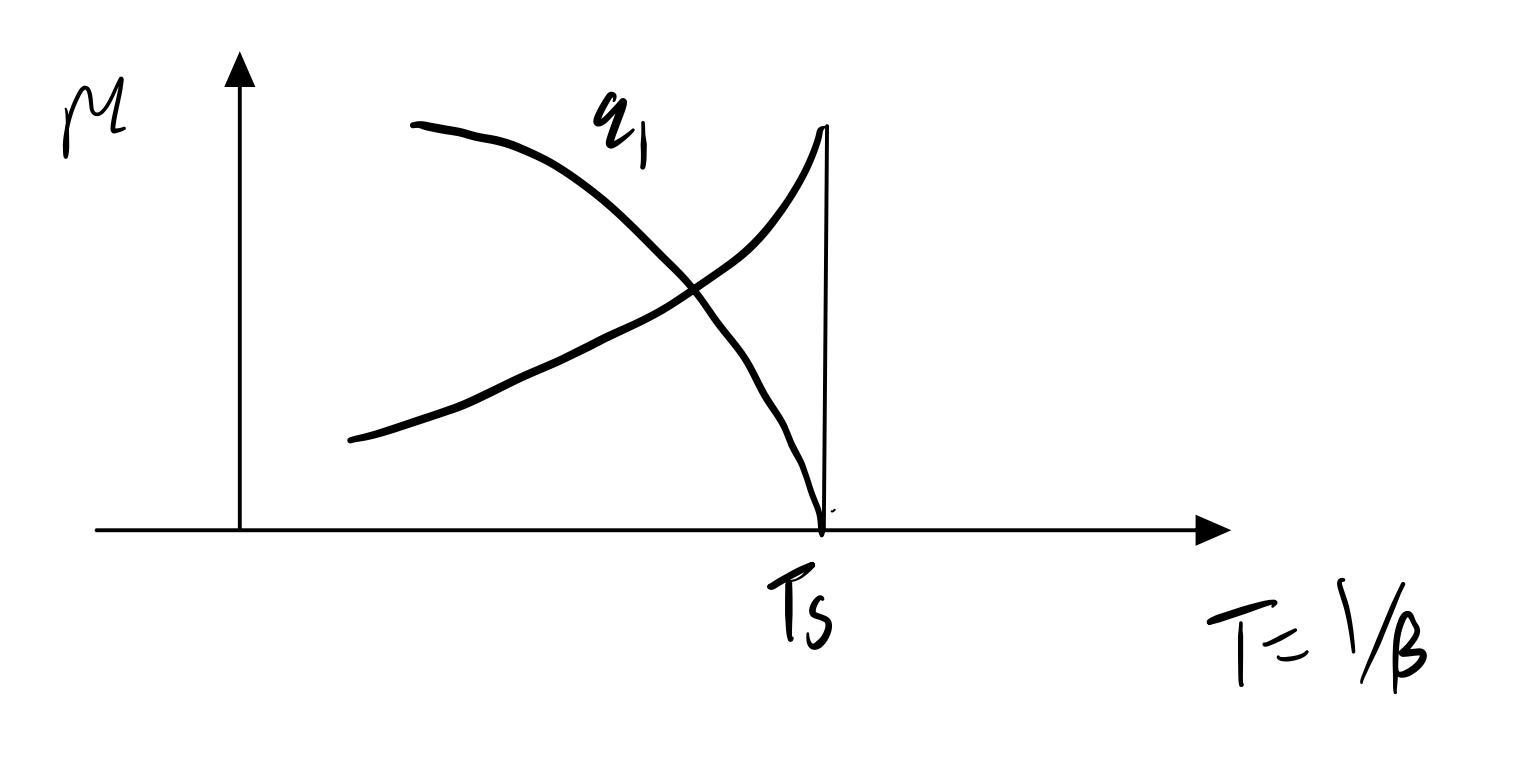
\includegraphics[scale=0.3]{Lectures/Figures/lec14-orderparam.png}
\end{center}

it is recommended to look at the homework problem before Friday - we'll come back to this last part, which we rushed a bit. What is the takehome message? The reason to writing down the odd model is that it is a mean field theory, and in MF models we are able to compute things easily from the saddle point. We are used to saddle points being very simple, but actually there is more complex structure to the saddle points than we are used to. But, if we look at finite $n$, we can visualize these solutions. We had a replica-symmetric solution, but the replica symmetry gets broken, leading to a fractal-like structure in the $Q$ matrix.